 \documentclass{sig-alternate-2}
   
   
 \conferenceinfo{GECCO'15,} {July 11-15, 2015, Madrid, Spain.}
 \CopyrightYear{2015}
 \crdata{TBA}
 \clubpenalty=10000
 \widowpenalty = 10000
    
    \title{Genetically-regulated Neuromodulation\\
    Facilitates Multi-Task Learning}
    
\numberofauthors{2}
\author{
\alignauthor
Sylvain Cussat-Blanc\\
\affaddr{University of Toulouse}\\
\affaddr{21 All\'ee de Brienne} \\
\affaddr{31042 Toulouse, France}
\email{cussat@irit.fr}
\and
\alignauthor
Kyle Harrington\\
\affaddr{Beth Israel Deaconess Medical Center}\\
\affaddr{Harvard Medical School}\\
\affaddr{02215 Boston, MA} \\
\email{kharrin3@bidmc.harvard.edu}
}

\date{}

\begin{document}
\maketitle

\begin{abstract}
In this paper, we use a gene regulatory network (GRN) to regulate a reinforcement learning controller, the State-Action-Reward-State-Action (SARSA) algorithm. The GRN modulates SARS's learning parameters: learning rate, discount factor, and memory depth. We have optimized GRNs with an evolutionary algorithm to regulate these parameters on specific problems but with no knowledge of problem structure. We show that GRN-regulated SARSA performs equally or better than the SARSA with fixed parameters. We then extend the GRN-regulated SARSA algorithm to multi-domain problem generalization, and show that GRNs trained on multiple problem domains can generalize to previously unknown problems with no further optimization. 
\end{abstract}

\category{I.2.6}{Learning}
\keywords{Reinforcement learning, Gene regulatory network, Parameter control, Multi-task Learning, Neuromodulation}

\section{Introduction}

Transfer and multi-task learning has recently been receiving attention within the reinforcement and machine learning communities \cite{Li2009,Taylor2009}. The ability to generalize between learnable tasks is a challenging ambition, that is far from fully solved, but is achievable, as evidenced by biological organisms capable of generalizing across multiple tasks. In this work we use an evolutionary algorithm to optimize gene-regulatory networks (GRNs) that dynamically tune the parameters of a reinforcement learning (RL) algorithm. This genetically-regulated neuromodulation (GRNM) extends previous results where we showed that GRNM can enhance the learning of agents beyond the performance of traditional fixed parameter RL \cite{Harrington2013}. We apply GRNM to additional problem classes, and show that GRNs evolved on agents learning a subset of problems can facilitate learning on previously unencountered problems. 

This paper is organized as follows. Firstly, we briefly summarize reinforcement learning and in more specifically the SARSA algorithm used in this study. Then, an introduction to gene regulatory network is given with the details on the computational model we use. Section 4 shows how we use the regulatory network for neuromodulation. Section 5 presents the four problems we use neuromodulation on and the results of GRNs trained specifically on each problem and the capacity of the GRNs to generalize their behavior to unknown problems.


%\section{SARSA Algorithm}
\section{Reinforcement Learning}
%%%%% from IJCNN %%%%
Reinforcement learning is a reward-based learning algorithm that allows agents
to learn from experience. More formally, reinforcement
learning (RL) is a mathematical framework for learning from a reward signal that
is derived from Bellman's equation for optimal control \cite{sutton1998introduction}. One of
the most important forms of RL is temporal-difference (TD) RL. TD-RL is a method
for learning optimal behavior from changes in state and reinforcement by error
prediction \cite{sutton1988learning}. TD-RL agents learn an expected return that will be
received after taking an action in any state. Strong correlations with this type of
error predictive behavior have been found in studies of dopamine neurons
\cite{schultz1993responses}. This line of research has continued and is now been
supported by fMRI data of reward processing for tastes, money, and love
\cite{haber2009reward}.

TD-RL is used to solve Markov decision processes, which are an extension of
Markov chains to problems framed in terms of state, action, and reward.
Reward signals are learned and encoded
in a table which associates action preferences with states. The basic
TD($\gamma$) algorithm updates one state-action association at a time which
prohibits sequence learning. Eligibility traces are used to associate reward
with sequences of actions by reinforcing a weighted history of most recent
actions. In this study the online version of TD-RL, SARSA (short for,
state-action-reward-state-action), is used. A review of the nuances of
reinforcement learning can be found in \cite{sutton1998introduction}.

%\subsection{SARSA Algorithm}

We include a few of the key equations from the SARSA algorithm. If we are in state,
$s_t$ at time $t$, then we will take some action $a_t$ which will bring us a
reward $r_t$. This action will also cause us to transition to a new state,
$s_{t+1}$. The SARSA algorithm learns a Q-function, which maps a value to each 
state-action pair, $(s_t,a_t)$. From each state multiple actions, $A_t$, may be taken
which may be a function of $s_t$ (for example, an obstacle may prevent an action
in a given state). Given an optimal Q-function the best action to take is
\begin{equation} argmin_{a_t \in A_t} Q(s_t,a_t).
\end{equation}
\noindent The Q-function is approximated by SARSA with the following update rule
\begin{eqnarray} 
& Q(s_t,a_t) \leftarrow Q(s_t,a_t)+ \nonumber \\ 
& \alpha \big[r_{t+1}+\gamma Q(s_{t+1},a_{t+1}) - Q(s_t,a_t)\big] 
\end{eqnarray}
\noindent where $\alpha$ is the learning rate, and $\gamma$ is the discounting
factor. Given only this update rule it can be difficult to compute the Q-value
for state-action pairs which indirectly contribute to obtaining a reward. This
update method propagates information only to the preceding state-action pair,
for those that are very distant from the reward, such as in the case of maze
solving problems, this can require a large number of repeated trials. However,
this problem of reward propagation can be partially alleviated by the use of
eligibility traces. Eligibility traces store an accumulating trace of
state-action pairs. The ``memory'' of these state-action pairs can be tuned with
the trace decay parameter $\lambda$. Eligibility traces are updated with
\begin{equation}
e_t(s,a) = 	\begin{cases}
			\gamma \lambda e_{t-1}(s,a) & \mbox{if } s \neq s_t \\ 
			\gamma \lambda e_{t-1}(s,a)+1 & \mbox{if }s = s_t \\
			\end{cases}
\end{equation} 
\noindent By combining the error predictive capabilities of SARSA with the
state-action sequence memory of eligibility traces we can amplify the effects
of our reward and speed up the learning process. When performing on-policy
learning it is important to ensure that a sufficient amount of exploration
occurs. To this end the $\epsilon$-greedy method is used, where a random
action is taken with $p(\epsilon)$, otherwise the agent's most preferred 
action is taken. However, the RL algorithm can still fail to capitalize on rarely
experienced rewards. 

\section{Gene Regulatory Network}
%%%% FROM IJCNN %%%%

Artificial gene regulatory networks (GRNs) are a class of biologically-inspired
algorithms. In living systems, gene regulatory networks are used within the cell
to control DNA transcription and, correspondingly, the phenotypic gene
expression. Although the inner workings of the cell are governed by a large collection
of complex machines, simplified models of cells as entities with protein sensors and actuators
both exhibit complex behavior and offer insights into natural systems \cite{Davidson2006}.
These protein sensors represent receptor molecules localized to the cellular membrane
which transduce external activity into excitatory and/or inhibitory regulatory signals.
Cells use external signals collected from protein sensors localized
on the membrane to activate or inhibit the transcription of the genes.

Our computational model uses an optimized network of abstract proteins. The inputs of the
agent are translated to protein concentrations that feed the GRN. Output
proteins regulate the reinforcement learning parameters previously described.
This kind of controller has been used in many developmental models of the
literature \cite{Joachimczak08, Doursat09, CussatBlanc2012a} and to control
virtual and real robots \cite{ziegler2001evolving, Nicolau10, Joachimczak10, CussatBlanc2012b}. 

In our model, a
gene regulatory network is defined as a set of proteins. Each protein has the
following properties:
\begin{itemize}
\item The \emph{concentration} is the quantity of each protein avalaible in the network. This concentration influences the regulation of other proteins: the higher the concentration, the higher the enhancing or the inhibiting impact on other proteins.

\item The protein \emph{tag} coded as an integer between 0 and $p$. The
	upper value $p$ of the domain can be changed in order to control the
	precision of the GRN. In Banzhaf's work, $p$ is equivalent to the size
of a site, 16 bits. 
% We have reduced the precision to 16 because the
% precision of the output values are not a particular requirement in that
% particular application.

\item The \emph{enhancer tag} coded as an integer between 0 and $p$. The
	enhancer tag is used to calculate the enhancing matching factor
	between two proteins.

\item The \emph{inhibitor tag} coded as an integer between 0 and $p$. The
	inhibitor tag is used to calculate the inhibiting matching factor
	between two proteins.

\item The \emph{type} determines if the protein is an \emph{input} protein, the
	concentration of which is given by the environment of the GRN and which
	regulates other proteins but is not regulated, an \emph{output} protein,
	the concentration of which is used as output of the network and which is
	regulated but does not regulate other proteins, or a \emph{regulatory}
	protein, an internal protein that regulates and is regulated by other
	proteins.

\end{itemize}

The dynamics of the GRN is calculated as follow. First, the affinity of a
protein $a$ with another protein $b$ is given by the enhancing factor
$u^{+}_{ab}$ and the inhibiting $u^{-}_{ab}$:
\begin{equation}
u^{+}_{ab}=p-|enh_a-id_b|~~;~~u^{-}_{ab}=p-|inh_a-id_b|
\end{equation}
where $id_x$ is the tag, $enh_x$ is the enhancer tag and $inh_x$
is the inhibiting tag of protein $x$.

The GRN's dynamics are calculated by comparing the proteins two by two using the
enhancing and the inhibiting matching factors. For each protein in the network,
the global enhancing value is given by the following equation:
\begin{equation}
g_i=\frac{1}{N}\sum_j^N{c_je^{\beta (u^{+}_{ij}-u_{max}^{+})}}~~;~~h_i=\frac{1}{N}\sum_j^N{c_je^{\beta (u^{-}_{ij}-u_{max}^{-})}}
\end{equation}
where $g_i$ (or $h_i$) is the enhancing (or inhibiting) value for a
protein $i$, $N$ is the number of proteins in the network, $c_j$ is the
concentration of protein $j$ and $u_{max}^{+}$ (or $u_{max}^{-}$) is the
maximum enhancing (or inhibiting) matching factor observed. $\beta$ is a
control parameter described hereafter.

The final modification of protein $i$ concentration is given by the following
differential equation:
\begin{equation}
\frac{dc_i}{dt}=\frac{\delta(g_i-h_i)}{\Phi}
\end{equation}
where $\Phi$ is a function that keeps the sum of all protein concentrations
equal to 1.

$\beta$ and $\delta$ are two constants that set up the speed of reaction of the
regulatory network. In other words, they modify the dynamics of the network. $\beta$
affects the importance of the matching factor and $\delta$ affects the level of
production of the protein in the differential equation. The lower both values,
the smoother the regulation. Similarly, the higher the values, the more sudden
the regulation. 


\section{Neuromodulation}
In living organisms, neuromodulators are neuropeptides or small molecules, such as dopamine and
serotonin. The production of these substances within the cell is controlled by
gene regulatory networks. Neuromodulators change the behavior of neural networks
within individual neurons, amongst neighboring neurons, or throughout the entire
network. Neuromodulation has been found to be pervasive throughout the brain,
and can have drastic consequences on the behavior of neurons and neuronal
circuits \cite{Destexhe2004,Marder2012,Marder2002}. We have already noted that the temporal difference learning algorithm for error
prediction has been observed in neural substrates \cite{Schultz1993}. An
extensive review of computational models of neuromodulation can be found in
\cite{Fellous1998}, and some recent models are reviewed in \cite{Marder2012}.
In this study we extend work on the evolution of neuromodulation \cite{Soltoggio2008,Harrington2013},
focusing on the relationship between evolved neuromodulatory
GRNs and reinforcement learning \cite{Harrington2013}. 

\subsection{Regulating parameters}
With the intention of focusing on the optimization of genetically-regulated neuromodulation, the physical mechanisms underlying neuromodulation are used as inspiration and the neuromodulation of reinforcement learning was optimized. Neuromodulation has been considered in the context of RL \cite{Doya2002,Schweighofer2003,Doya2008}, but this previous work has not focused on the implications of neuromodulation on problem solving capacity. In this work we utilize the artificial gene regulatory network presented in the previous section to regulate the learning parameters of the SARSA algorithm. Three learning parameters are considered: the learning rate $\alpha$, the discount factor $\gamma$ and the memory depth $\lambda$.

To do so, the GRN uses three inputs that describe the current performance of the agent in the environment. They have been chosen to be problem-independent as one of our goals is to define a problem-independent neuromodulation architecture to minimize problem-specific adjustments. The first input describes the duration from the beginning of current episode: the concentration of this first input protein increases with the time spent in each learning episode. The concentration $C_{I_1}(t)$ of this input protein at time step $t$ is calculated as follows:
\begin{equation}
C_{I_1}(t)=e^{-\frac{t^2}{t_{max}^2}}
\end{equation}
where $t_{max}$ is the expected duration of an episode. The second output protein's concentration $C_{I_2}(t)$ describes the quality of the current sequence of actions in term of rewards, smoothed on 25 steps:
\begin{eqnarray}
C_{I_2}(t)=\frac{\sum\limits_{s=1}^{25}{\Big((25-s)\times q_s(t-1)\Big)}}{\sum\limits_{s=1}^{25}s} \\
\text{with }q_s(t)=
\begin{cases}
1+1000\frac{Q.e}{Q.Q*e.e} & \text{ if} \frac{Q.e}{Q.Q*e.e}>0.4995\\
0 & \text{ otherwise}
\end{cases}\nonumber
\end{eqnarray}
where $e$ is the eligibility trace and $Q$ is the Q-function, both described in Section \ref{sec:RL}. The aim of this input is to capture the quality of the current state history relative to previous experiences. Finally, the third input protein's concentration $C_{I_3}(t)$ informs the GRN about the 25-step smoothed average reward the agent can obtain in its current state:
\begin{equation}
C_{I_3}(t)=\frac{\sum\limits_{s=1}^{24}{\Big((25-s)\times C_{I_3}(t-s)\Big)}+25\times \sum\limits_{r_e\in e}{r_e}}{\sum\limits_{s=1}{25}s}
\end{equation}
where $e$ is the eligibility trace. This input encodes the frequency that the agent has reentered the same state. 

In addition to these inputs, the GRN uses four output proteins to regulate the learning parameters:
\begin{itemize}
\item the output protein $O_{n}$, which concentration $C_{n}$ normalizes the concentration of other outputs\footnote{This is generally used in regulatory networks to obtain output values in $[0, 1]$.},
\item the output protein $O_{\alpha}$ of concentration $C_{\alpha}$, which provides the value for $\alpha$ to the SARSA algorithm with $\alpha=C_{\alpha}/(C_\alpha+C_{n})$,
\item the output protein $O_\gamma$ of concentration $C_{\gamma}$, which provides the value for $\gamma$ to the SARSA algorithm with $\gamma=C_{\gamma}/(C_\gamma+C_{n})$,
\item the output protein $O_\lambda$ of concentration $c_{\lambda}$, which provides the value for $\lambda$ to the SARSA algorithm with $\lambda=C_{\lambda}/(C_\lambda+C_{n})$.
\end{itemize}

As depicted by figure \ref{fig:GRNSARSA}, the GRN updates SARSA's learning parameters at every time step, before SARSA updates its internal variables and prediction. The GRN returns the learning parameters SARSA uses for its own decision step.

\begin{figure}
\center
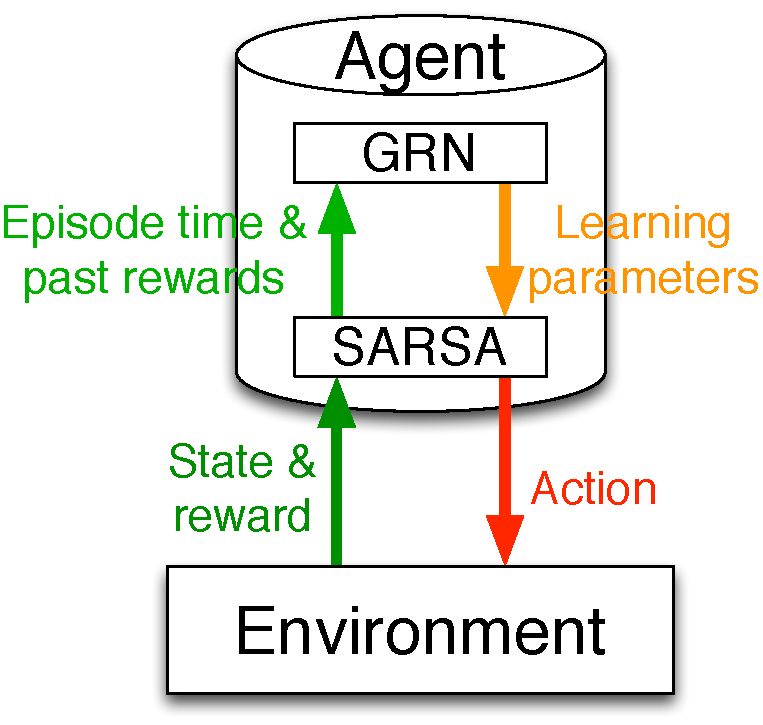
\includegraphics[width=0.7\linewidth]{GRNSARSA.pdf}
\caption{At every time step, SARSA updates the GRN inputs. The GRN returns updated learning parameters that will be used by the SARSA algorithm.}\label{fig:GRNSARSA}
\end{figure}

%%% Problem figure from experiences %%%
\begin{figure*}[ht!]
\begin{minipage}[t]{0.31\linewidth}
\center
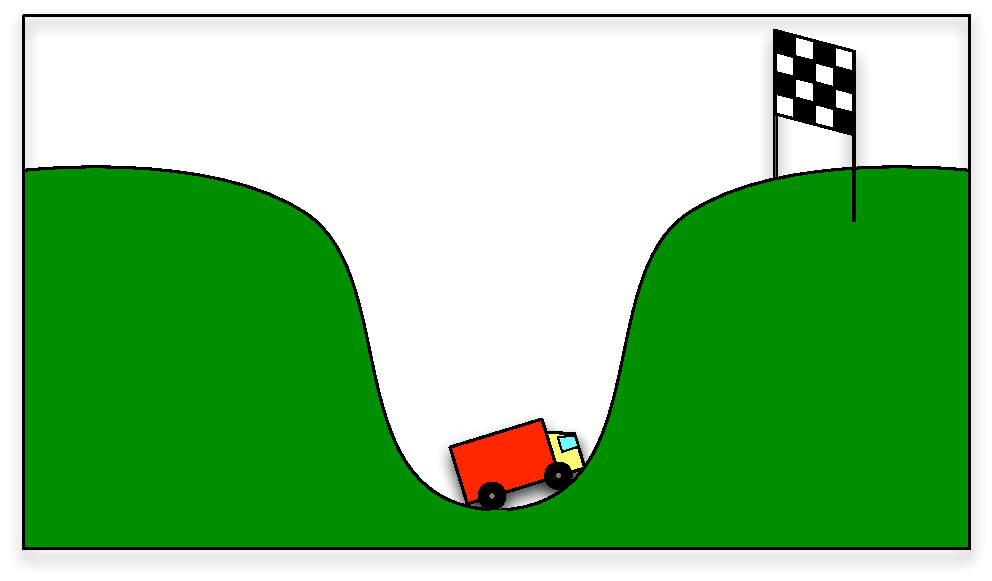
\includegraphics[height=3.2cm]{MC_problem.pdf}
\caption{Mountain Car
%In the mountain car problem, a car must escape from a valley. It cannot climb the hill without moving backward first to gain speed. The agent receives a reward only when it escapes.
}\label{fig:MC:problem}
\end{minipage}
\hspace{0.1mm}
\begin{minipage}[t]{0.25\linewidth}
\center
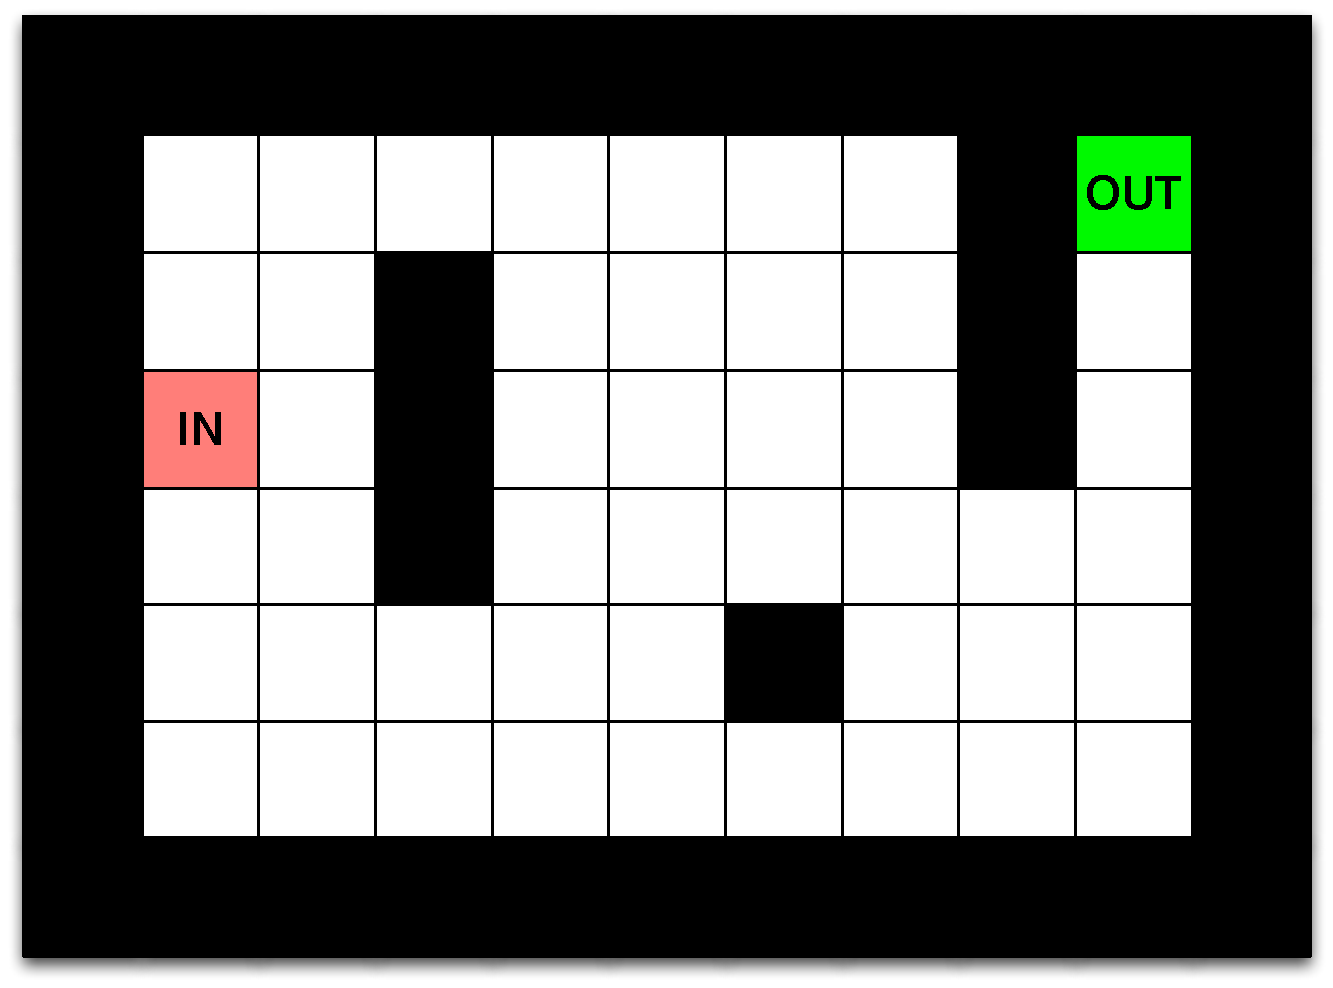
\includegraphics[height=3.2cm]{MZ_problem.pdf}
\caption{Maze
%In the maze problem, the agent's task is to find its way in a maze from start (in red) to finish (in green). The agent receives a reward only when it escapes.
}\label{fig:MZ:problem}
\end{minipage}
\hspace{0.1mm}
\begin{minipage}[t]{0.22\linewidth}
\center
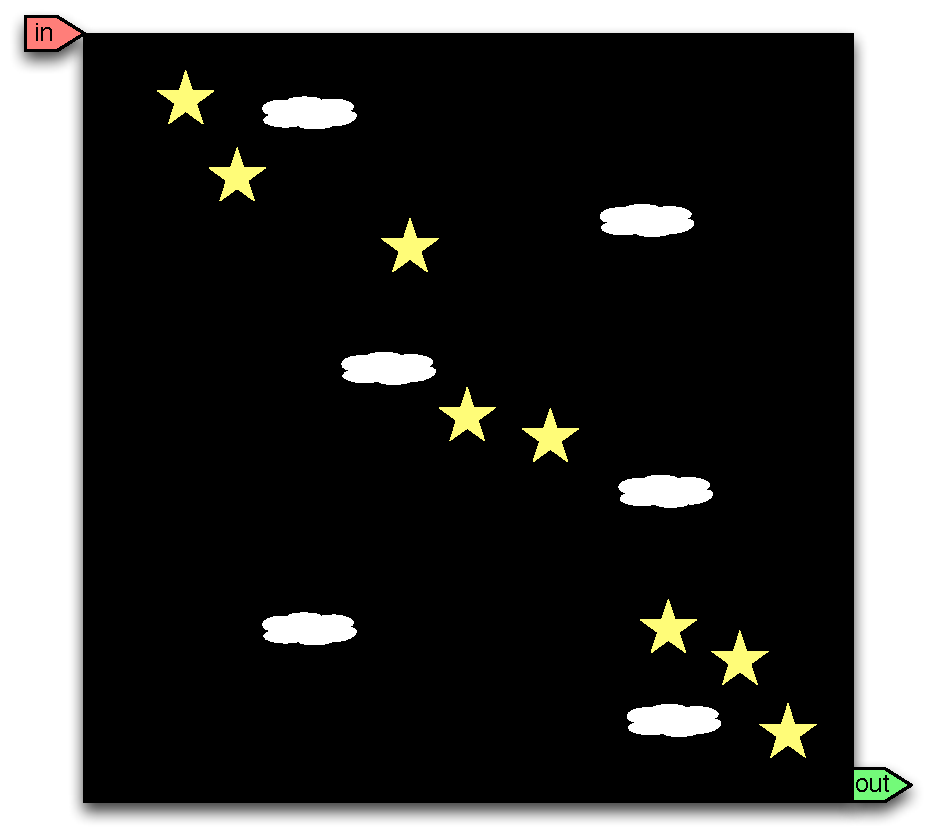
\includegraphics[height=3.2cm]{PW_problem.pdf}
\caption{Puddle World
%In the puddle world problem, the agent must navigate without sensor information with stochastic movements from start to finish. Rewards are given all along its exploration (stars) and when it escapes.
}\label{fig:PW:problem}
\end{minipage}
\hspace{0.1mm}
\begin{minipage}[t]{0.19\linewidth}
\center
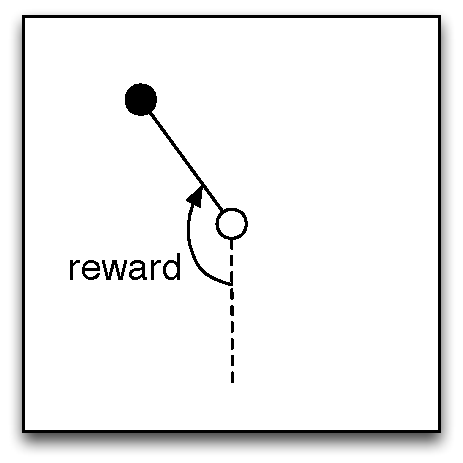
\includegraphics[height=3.2cm]{ACP_problem.pdf}
\caption{Acrobat
%In the acrobat problem, the agent has to balance a pendulum in a perfectly upright position. The reward is given by the cosine of the angle between the pendulum and the resting position.
}\label{fig:ACP:problem}
\end{minipage}
\end{figure*}

\subsection{GRN Optimization}
Before a gene regulatory network can be used for successful neuromodulation, the GRN must be optimized. In this paper, we use an evolutionary algorithm inspired by the NEAT algorithm \cite{stanley2002evolving}, but adapted for GRNs called GRNEAT \cite{cussatblanc2015grneat}. GRNEAT incorporates three key features:
(1) \emph{initialization} of the algorithm  - as opposed to initializing with network sizes randomly sampled from the complete distribution, only small networks are used in the initial population so as to allow for a more progressive complexification,
(2) \emph{speciation} protects newly appeared solutions by giving them some time to optimize their structures before competing with the whole population, and
(3) \emph{alignment crossover} uses of a distance metric between proteins to maintain subnetwork architecture during the crossover operation.
This modified algorithm has been shown to converge faster and to better solutions than standard genetic algorithms. More details on GRNEAT can be found in \cite{cussatblanc2015grneat}.

During optimization, each GRN is evaluated independently on a given problem with 25 reruns in order to reduce the effect of stochasticity on fitness. As fitness is problem dependent, more detail is provided in the corresponding experiment sections. To avoid any memory bias, SARSA is completely reset before each evaluation. The parameters used for GRNEAT in this work are given by Table~\ref{tab:GREAT:params}, and are consistent for all problems. 

\begin{table}
\center
\begin{tabular}{rl}
Parameter			& value 					\\\hline
Population size		& 500					\\
Initial duplicates		& 19					\\
Speciation threshold 	& 0.15					\\
Species min size		& 15					\\
Selection				& 3-players tournament	\\
Crossover rate		& 0.2					\\
Mutation rate			& 0.8					\\
\end{tabular}
\caption{GRNEAT parameters used for evolution.}\label{tab:GREAT:params}
\end{table}





\section{Experiences}
\subsection{Problems}
\subsubsection{Mountain Car}
\begin{figure}
\center
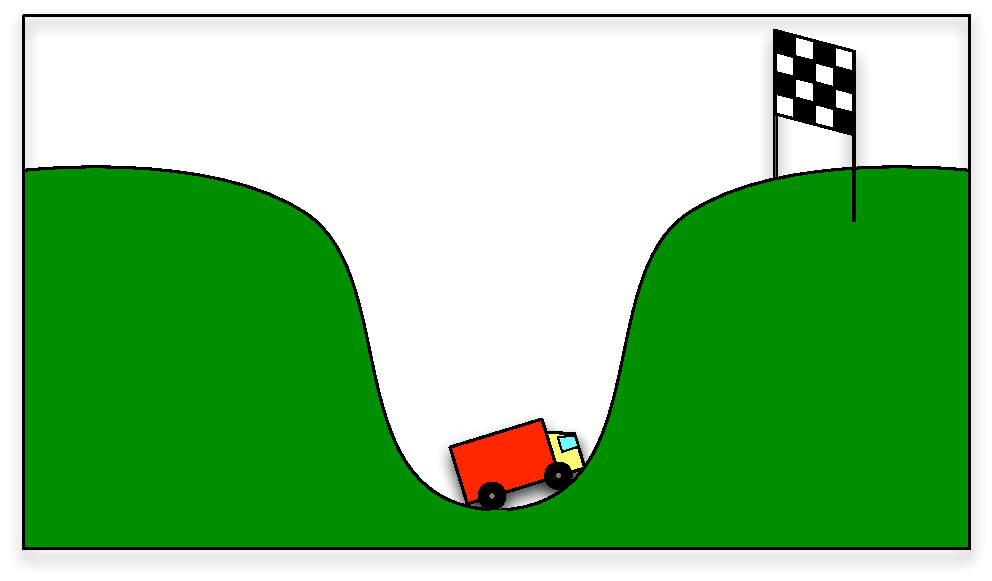
\includegraphics[width=0.75\linewidth]{MC_problem.pdf}
\caption{In the mountain car problem, a car must escape from a valey. It cannot climp the hill without moving backward first to gain speed. The agent receives a reward only when it escapes.}\label{fig:MC:problem}
\end{figure}

\subsubsection{Maze}
\begin{figure}
\center
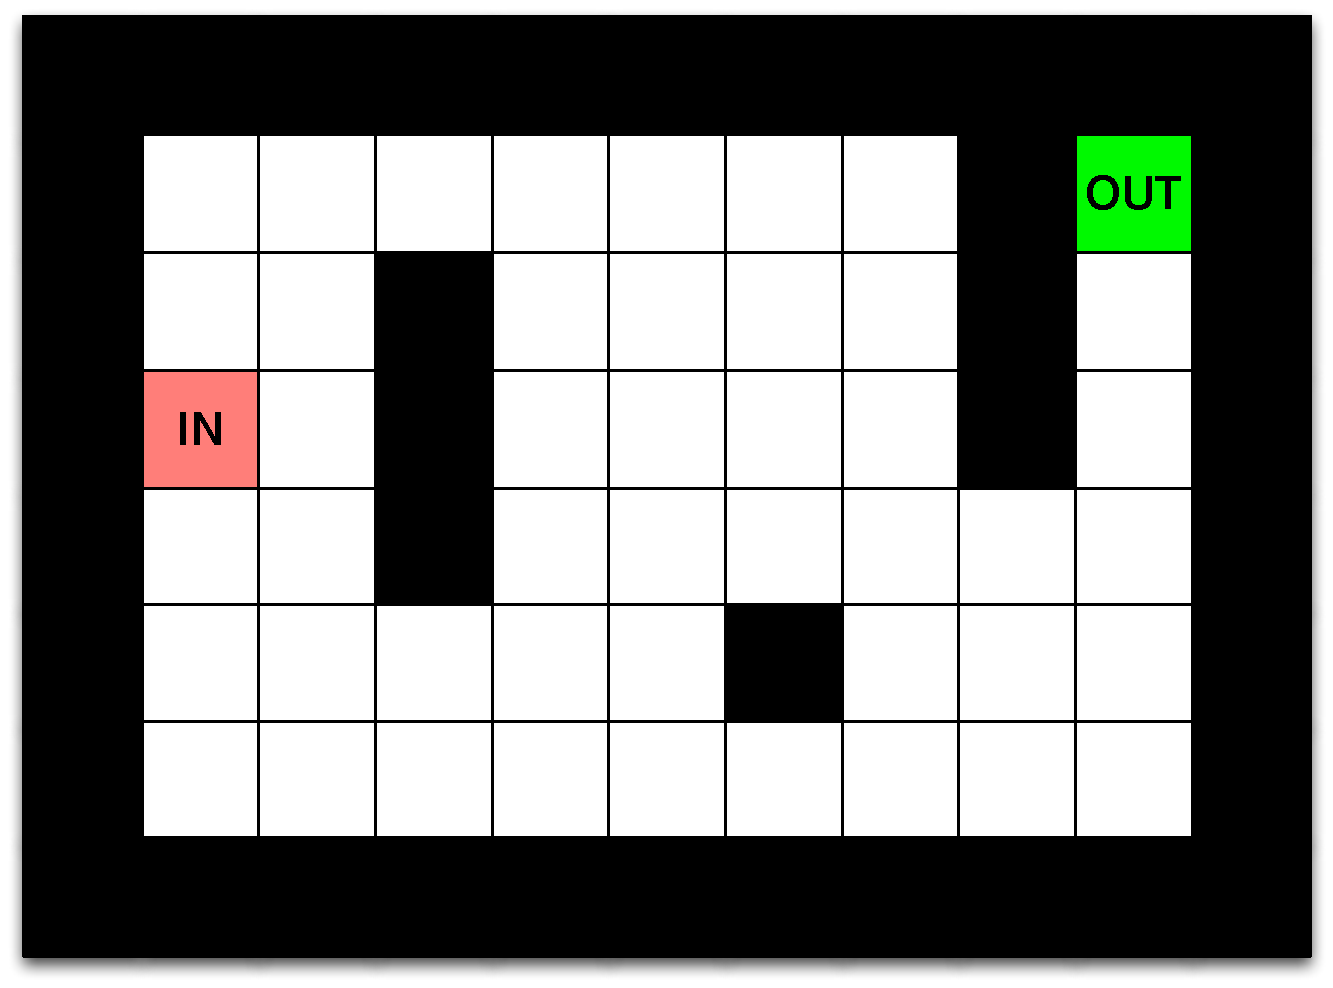
\includegraphics[width=0.75\linewidth]{MZ_problem.pdf}
\caption{In the maze problem, the agent have to find its way in a maze from the start (in red) to the end (in green). The agent receives a reward only when it escapes.}\label{fig:MC:problem}
\end{figure}

\subsubsection{Puddle World}
\begin{figure}
\center
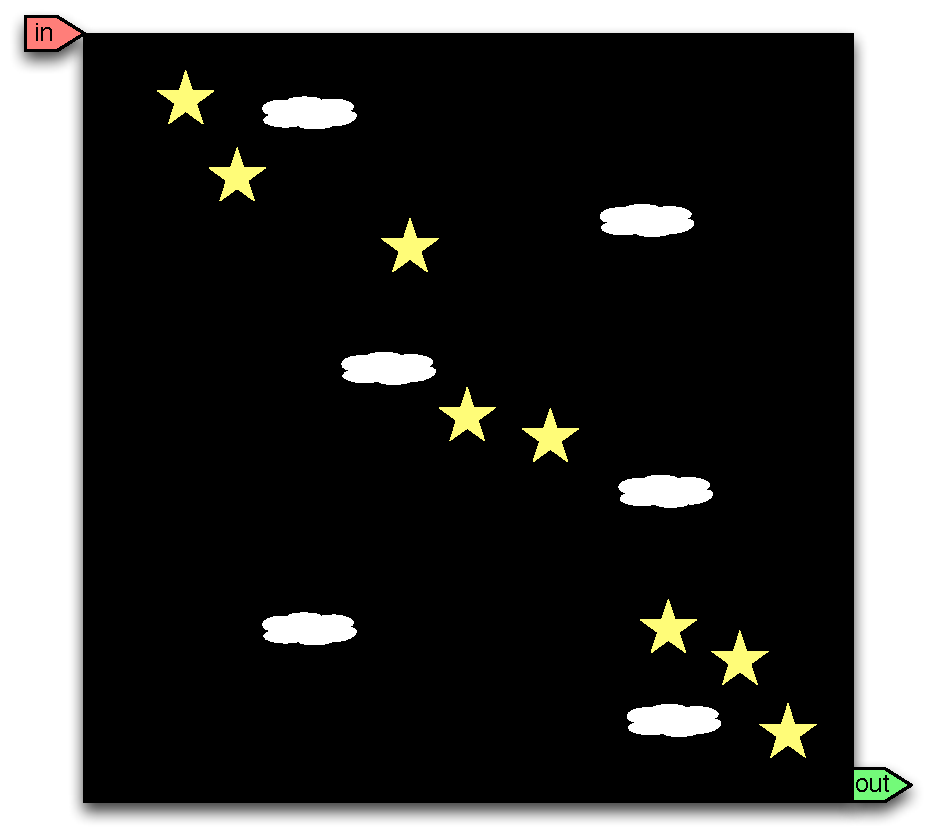
\includegraphics[width=0.75\linewidth]{PW_problem.pdf}
\caption{In the puddle world problem, the agent have to find its way in a dark environment from the start (in red) to the end (in green). Local rewards are given all along its exploration and when it escapes.}\label{fig:MC:problem}
\end{figure}

\subsubsection{Actor critic pendulum}
\begin{figure}
\center
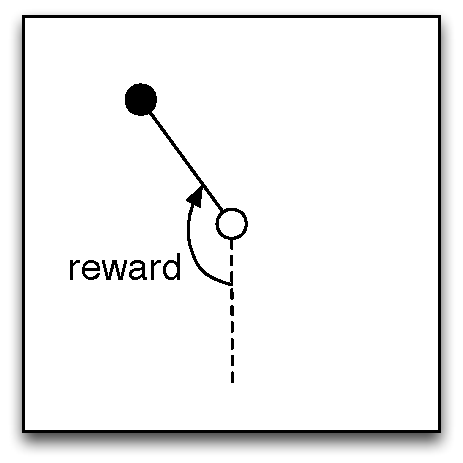
\includegraphics[width=0.5\linewidth]{ACP_problem.pdf}
\caption{In the actor critic pendulum, the agent has to balance a pendulum to the highest possible position. The reward is given by the cosinus of the angle between the pendulum and the resting position.}\label{fig:MC:problem}
\end{figure}


\subsection{Training GRN on one specific problem}
In this first experience, we have trained our GRN-based neuromodulation model independently on each problem above mentionned. To evaluate the gain provided by neuromodulation, we first determine the best fixed learning parameter to use with SARSA on each problem. We use parameter sampling on $\alpha$, $\gamma$ and $\lambda$ in $[0, 1]$ with 0.0714 steps (15 evaluations). Each evaluation is averaged on 10 replicates in order to reduce the randomness of the problems. At the end of the parameter sampling stage, we chose the best fixed learning parameters for a given problem by selecting the tuple with the highest fitness. These parameters are given in table \ref{tab:SARSAFixedParams}.

\begin{table}
\begin{tabular}{c|ccc}
%\cline{2-4}
					& $\alpha$	& $\gamma$	& $\lambda$	\\\hline
Mountain car			& 0.071429	& 1.0		& 0.928571 	\\%\hline
Maze				& 1.0		& 0.928571	& 0.928571	\\%\hline
Puddle world			&  0.057142	& 0.928571	& 0.5		\\%\hline
Actor critic pendulum	& 0.05		& 0.928571	& 0.785714	\\%\hline
\end{tabular}
\caption{Fixed learning parameters for SARSA obtained by parameter sampling}\label{tab:SARSAFixedParams}
\end{table}

\subsubsection{Mountain car}
First, the GRN is trained on Mountain car. Figure \ref{fig:MC:Convergence} shows the convergence curve of the genetic algorithm on this particular problem. We can observe that the best GRN is found very quickly (green curve) before being slowly optimized to regulate the learning parameters more efficiently. Figure \ref{fig:MC:GRNBehavior} plots the behavior of the best GRN obtained after 150 iterations. This figure plots the input protein concentrations and the three learning parameters calculated by the gene regulatory network. The GRN maintains the parameter values almost constant over the time except at the beginning of each episode where $\alpha$ and $\gamma$ are increase to explore more, certainly due to the novelty of the environment. In this experience, it has also to be noticed that $\lambda$ is kept to zero all over time. On this simple problem, memory might not be necessary. 

This GRN is then compared to the SARSA algorithm with fixed learning parameters on 100 independent reruns of mountain car with different different random seed. The point is to evaluate the capacity of both approaches to handle the noise generated by randomness. Figure \ref{fig:MC:GRNvsSARSA} shows the results obtained for each episode averaged on the 100 runs. We can observe that neuromodulation with GRN trained on the mountain car (in green) beats SARSA with fixed parameters (in red) on every episodes. More specifically, the first episodes (from 1 to 3) show that GRN-based neuromodulation learns faster than SARSA and later episodes (from 3 to 25) show that neuromodulation solves the problem faster than SARSA.

\begin{figure}
\center
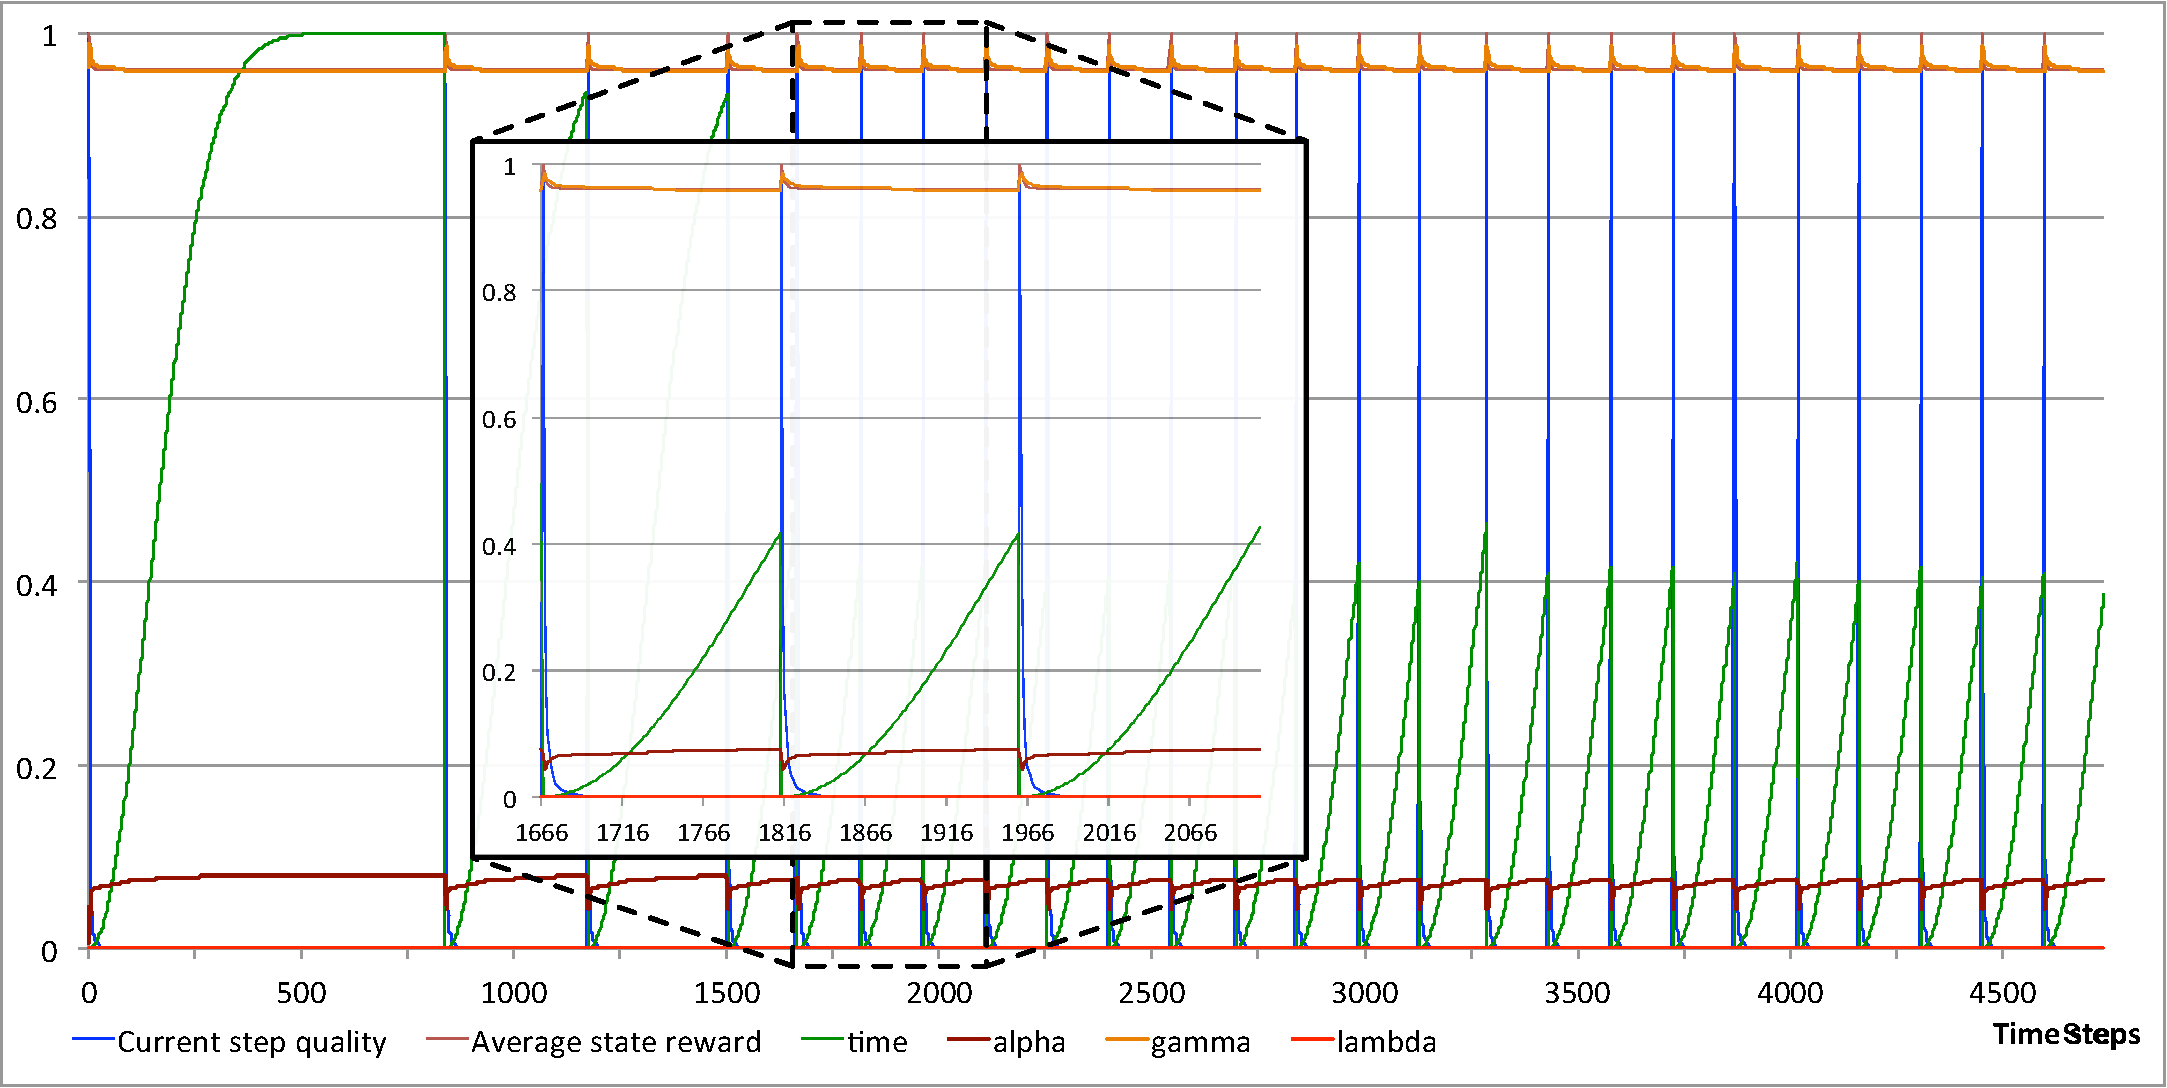
\includegraphics[width=\linewidth]{MC_GRNBehavior.pdf}
\caption{Moutain car: Regulation of the learning parameters of the best GRN obtained.}\label{fig:MC:GRNBehavior}
\end{figure}

\begin{figure}
\center
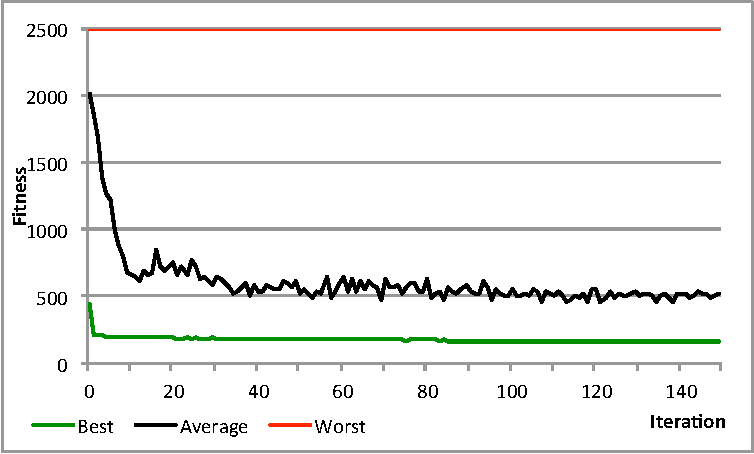
\includegraphics[width=0.75\linewidth]{MC_convergence.pdf}
\caption{Mountain car: Convergence curve of the genetic algorithm (lower is better - time to escape the valley).}\label{fig:MC:Convergence}
\end{figure}

\begin{figure}
\center
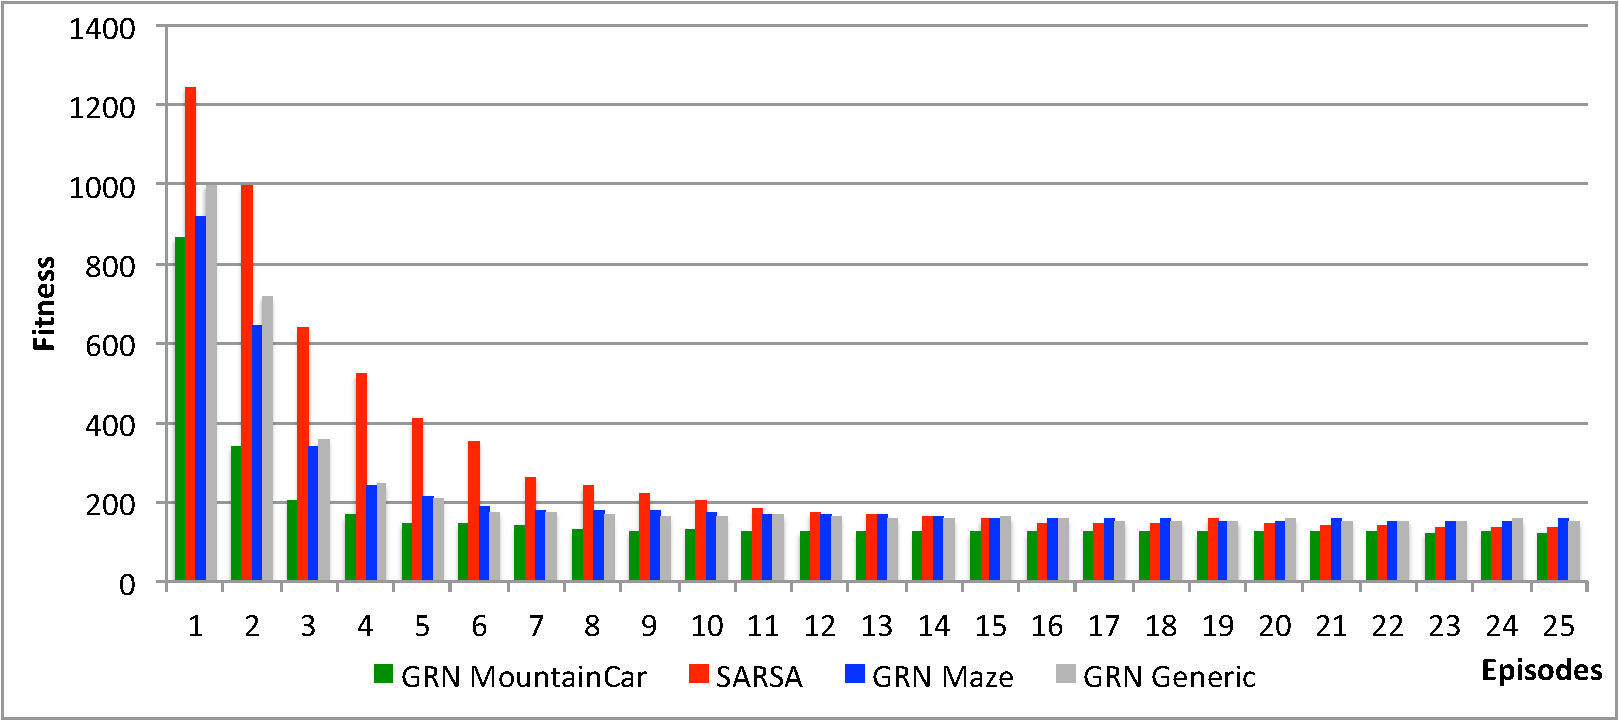
\includegraphics[width=\linewidth]{MC_GRNvsSARSA.pdf}
\caption{Mountain car: Comparison of the fitnesses per episode (abscissa) obtained by our neuromodulation with a GRN trained on mountain car (green), with a GRN trained on maze (blue) and with parameter-fixed SARSA (red). Results are averaged on 100 independent runs.}\label{fig:MC:GRNvsSARSA}
\end{figure}

\subsubsection{Maze}
The same procedure has been used to evolve a gene regulatory network to regulate SARSA's learning parameters on the maze problems. Figure \ref{fig:MZ:GRNBehavior} presents the behavior of the best GRN obtained after evolution. The regulation broadly differs from the one obtained on the mountain car problem. This GRN starts with very high values for all learning parameters with the aim to explore widely the environment. Then, with sucessfull episodes incoming, the learning rate $\alpha$ and the memory depth $\lambda$ decrease to exploit the behavior learnt during the first scenarios. $\gamma$ is kept very high all along the simulation.

When compared to parameter-fixed SARSA (figure \ref{fig:MZ:GRNvsSARSA}), we can observe that the GRN is learning faster than SARSA (episodes 2 to 5) due to its high learning rate at the begining of the simulation. However, the avantage turns to fixed-parameter SARSA in the remaining episodes: SARSA is doing slightly better than neuromodulation from episode 6 to the end.

\begin{figure}
\center
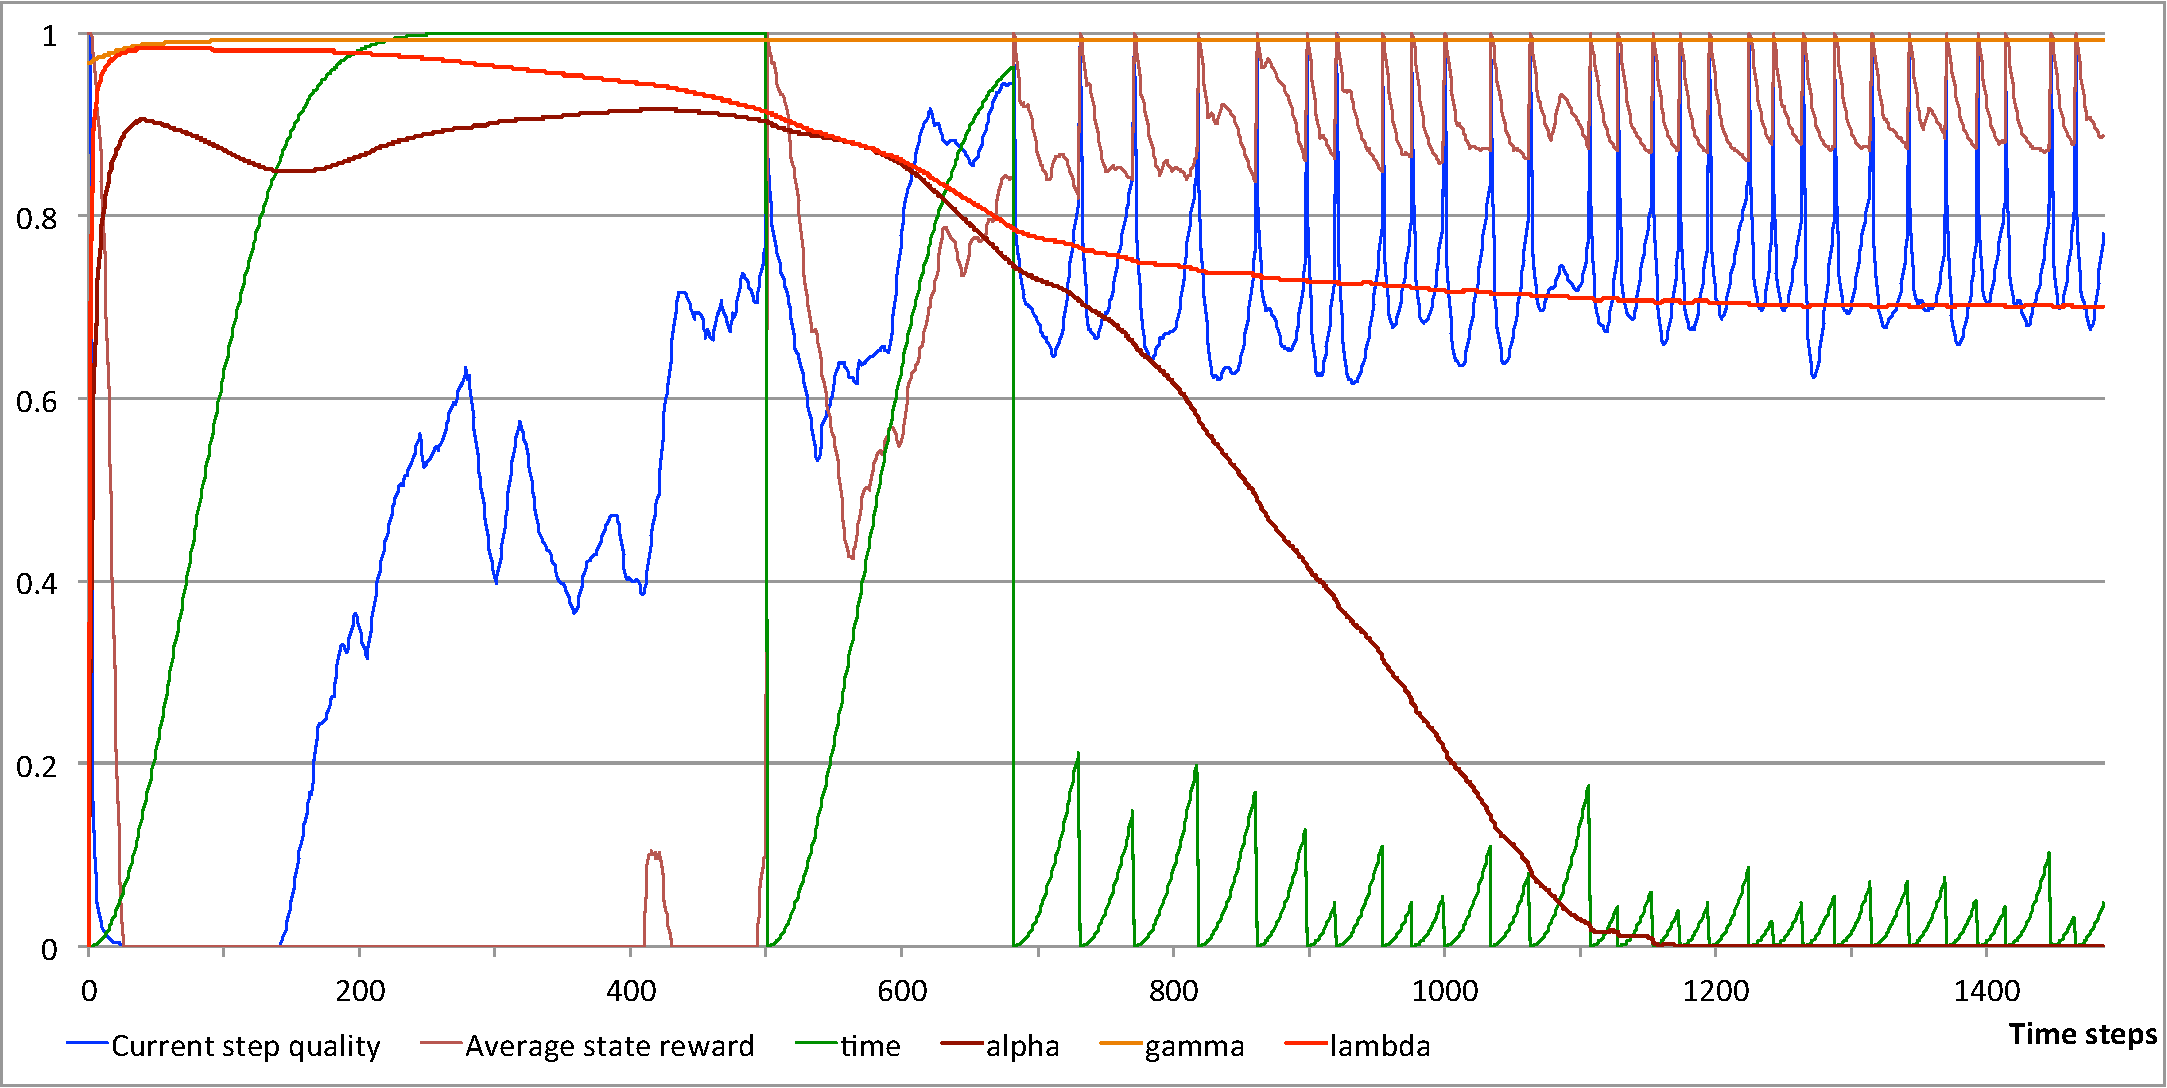
\includegraphics[width=\linewidth]{MZ_GRNBehavior.pdf}
\caption{Maze: Regulation of the learning parameters of the besst GRN obtained.}\label{fig:MZ:GRNBehavior}
\end{figure}

\begin{figure}
\center
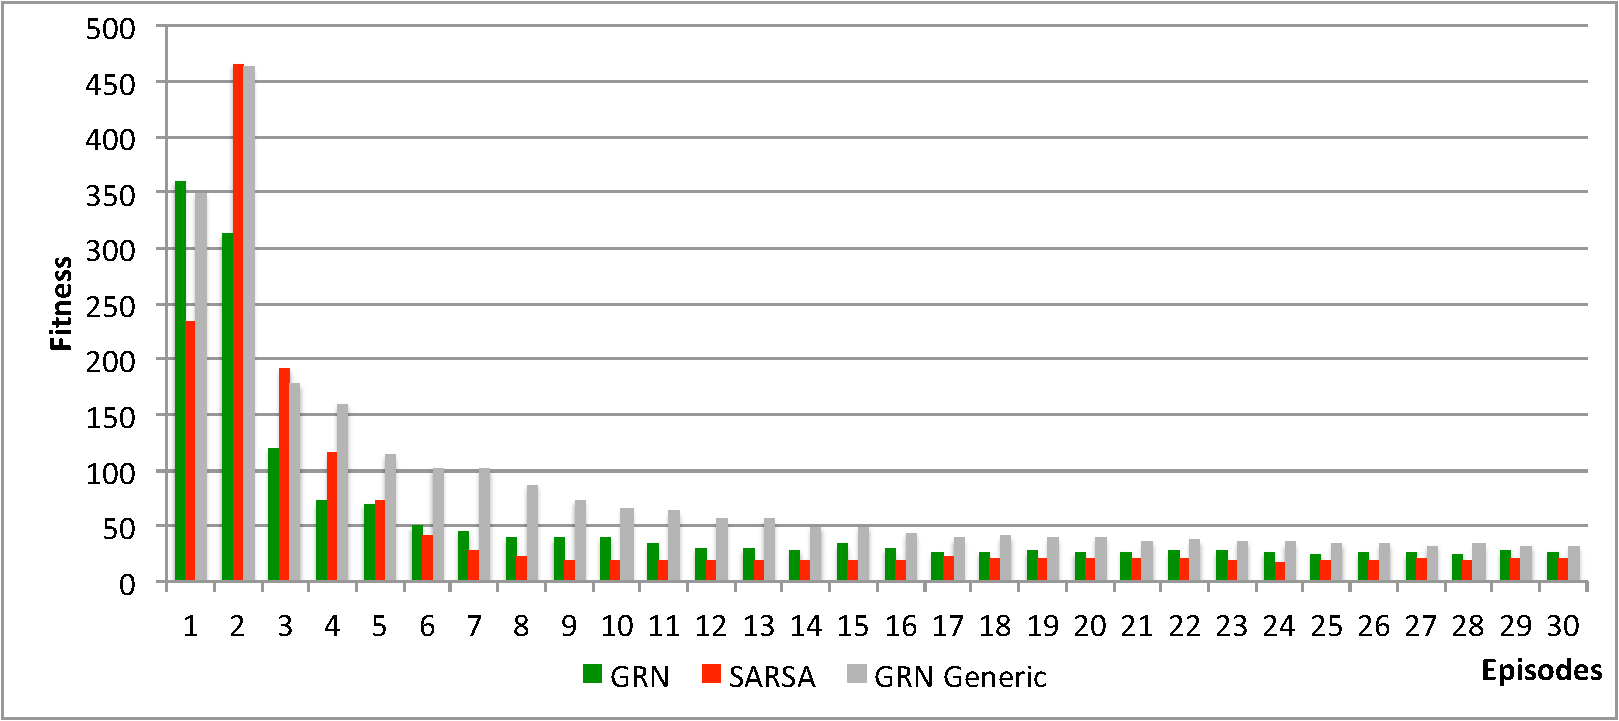
\includegraphics[width=\linewidth]{MZ_GRNvsSARSA.pdf}
\caption{Maze: Comparison of the fitnesses per episode (abscissa) obtained by our neuromodulation with a GRN trained on maze (green) and with parameter-fixed SARSA (red). Results are averaged on 100 independent runs.}\label{fig:MC:GRNvsSARSA}
\end{figure}


\subsubsection{Puddle world}

\subsubsection{Actor critic pendulum}

\subsection{Generalization of the regulation}

\section{Conclusion}
% discrete problems seem harder for the GRN... we need to say that in the conclusion

In this paper, we proposed to evolve a gene regulatory network to control reinforcement learning paramaters on four state-of-the-art problems. We have evolve GRN specificially on each task, which produce better or equivalent results than parameter-fixed SARSA on average. In all cases, the worst case scenario is always better handle by GRN-based neuromodulation because of its capacity to modify the learning parameters on-the-fly to escape dead ends. 

In addition, the GRN evolved on the maze as well as a generic GRN have been tested on the problems and provides encouraging results with no further learning. Once again, the worst case scenario is better handled by neuromodulation with generic GRNs than without neuromodulation. However, generic GRNs are not as good as GRN specifically evolved on each task. Other inputs might be usefull to the GRN to estimate the quality of the current neuromodulation and the quality of the agent behavior. Finding a generic GRN able to perfectly modulate the learning parameter would make possible not to evolve the GRN anymore and use it as is on all possible problems. That would make the parameter sampling phase of reinforcement learning out of date.

%\section{Future Work}
As was noted in \cite{Schweighofer2003}, neuromodulation is neither problem nor RL-algorithm specific, thus future work may investigate the application of GRN-neuromodulation on alternative RL algorithms. We have shown that a simple feedback controller can optimize community features of agent-based swarm simulations, the use of GRN-based neuromodulation is likely to further optimize these environmental controllers \cite{Gold2014}. Having a problem-independent and algorithm-independent neuromodulation architecture would save a large amount of set up for both the problem and the algorithm.

\textbf{Acknowledgements:} Kyle Harrington is supported by NIH grant 2T32HL007893-16A1.


\bibliographystyle{abbrv}
\bibliography{bibtex}


\end{document}

